\documentclass{article}
\usepackage[utf8]{inputenc}
\usepackage[spanish]{babel}
\usepackage{geometry}
\geometry{margin=2.5cm}
\usepackage{amsmath}
\usepackage{xcolor}
\usepackage{graphicx}

\begin{document}

\title{Métodos de Optimización -- 28 de mayo de 2025}
\author{Universidad Nacional del Altiplano\\
Facultad de Ingeniería Estadística e Informática\\
Docente: Fred Torres Cruz}
\date{}

\maketitle

\noindent Apellidos y Nombres: Caceres Tacora Lizbeth Estefany \\
Código: 230042

\section{Evaluación Teórica}

\begin{enumerate}
\item ¿Cuál de las siguientes afirmaciones describe mejor una función lineal?
\begin{enumerate}
\item Es una función que tiene exponentes no lineales
\item Es una función que se representa gráficamente como una curva
\item \colorbox{yellow}{Es una función cuya gráfica es una línea recta}
\item Es una función que involucra productos de variables
\item Es una función con términos cuadráticos
\end{enumerate}

\item En programación lineal, ¿cuál es el principal objetivo de las restricciones?
\begin{enumerate}
\item Minimizar el número de variables en la función objetivo
\item \colorbox{yellow}{ Establecer las condiciones bajo las cuales se deben encontrar soluciones}
\item Maximizar el valor de la función objetivo
\item Aumentar el número de soluciones posibles
\item Simplificar el cálculo de la función objetivo
\end{enumerate}

\item ¿Qué concepto define el conjunto de todas las soluciones posibles que satisfacen las restricciones de un problema de optimización?
\begin{enumerate}
\item \colorbox{yellow}{Región factible}
\item Función objetivo
\item Solución degenerada
\item Solución óptima
\item Solución no acotada
\end{enumerate}

\item ¿Cuál de los siguientes es un objetivo típico en los problemas de optimización?
\begin{enumerate}
\item Hallar el máximo local de una función
\item \colorbox{yellow}{Encontrar el valor mínimo o máximo de una función objetivo sujeta a restricciones}
\item Minimizar el número de variables
\item Encontrar soluciones inexactas para ecuaciones no lineales
\item Resolver integrales definidas
\end{enumerate}

\item ¿Qué condición debe cumplirse para que un sistema de ecuaciones lineales tenga una única solución?
\begin{enumerate}
\item El determinante de la matriz asociada debe ser cero
\item El sistema debe ser homogéneo
\item \colorbox{yellow}{El determinante de la matriz asociada debe ser distinto de cero}
\item El sistema debe ser dependiente
\item No debe haber ninguna restricción adicional
\end{enumerate}

\item Una empresa produce sillas ($x$) y mesas ($y$). Cada silla genera una utilidad de 40 y cada mesa 60. Si la función objetivo es:
\[
\text{Maximizar } Z = 40x + 60y
\]
¿Qué representa el valor 60?
\begin{enumerate}
\item El costo de producir una mesa
\item \colorbox{yellow}{La utilidad unitaria por cada mesa vendida}
\item El número máximo de mesas que se pueden producir
\item El tiempo necesario para producir una mesa
\item El precio de venta de una mesa
\end{enumerate}

\item ¿Qué tipo de función es típicamente la función objetivo en programación lineal?
\begin{enumerate}
\item Una función cuadrática
\item Una función polinómica
\item \colorbox{yellow}{Una función lineal}
\item Una función logarítmica
\item Una función exponencial
\end{enumerate}

\item ¿Qué diferencia hay entre restricciones de igualdad y restricciones de desigualdad en programación lineal?
\begin{enumerate}
\item Las restricciones de igualdad no afectan el resultado
\item \colorbox{yellow}{\parbox{\linewidth}{Las restricciones de desigualdad limitan el conjunto factible, mientras que las de igualdad lo definen completamente.}}

\item Solo las restricciones de desigualdad son necesarias para resolver el problema
\item Las restricciones de igualdad simplifican el cálculo de la función objetivo
\item Las restricciones de desigualdad no limitan el espacio de soluciones
\end{enumerate}

\item ¿Cuál de los siguientes no es un tipo de restricción en programación lineal?
\begin{enumerate}
\item Restricciones de igualdad
\item Restricciones de desigualdad
\item Restricciones implícitas
\item \colorbox{yellow}{Restricciones no lineales}
\item Restricciones de viabilidad
\end{enumerate}

\item En la teoría de la optimización, el tiempo de ejecución de un algoritmo depende principalmente de:
\begin{enumerate}
\item El número de variables del problema
\item El número de soluciones óptimas
\item El tipo de función objetivo
\item La cantidad de restricciones
\item \colorbox{yellow}{La complejidad del algoritmo utilizado}
\end{enumerate}
\end{enumerate}

\section{Evaluación Práctica}

\textbf{Pregunta 1:}

Una empresa realiza análisis de datos de redes sociales para predecir tendencias en el mercado local. El departamento de análisis utiliza dos tipos de servidores: Servidor A y Servidor B. El Servidor A puede procesar 500 GB de datos en 10 horas, mientras que el Servidor B procesa 300 GB en 8 horas. Ambos servidores tienen un límite máximo de funcionamiento diario de 12 horas, y el almacenamiento total disponible en la empresa es de 4000 GB por día. Además, el costo de energía por hora en el Servidor A es de 50 soles y en el Servidor B es de 30 soles. El objetivo es maximizar la cantidad de datos procesados al día sin superar el presupuesto de 1200 soles diarios en energía.

\begin{figure}[h]
    \centering
    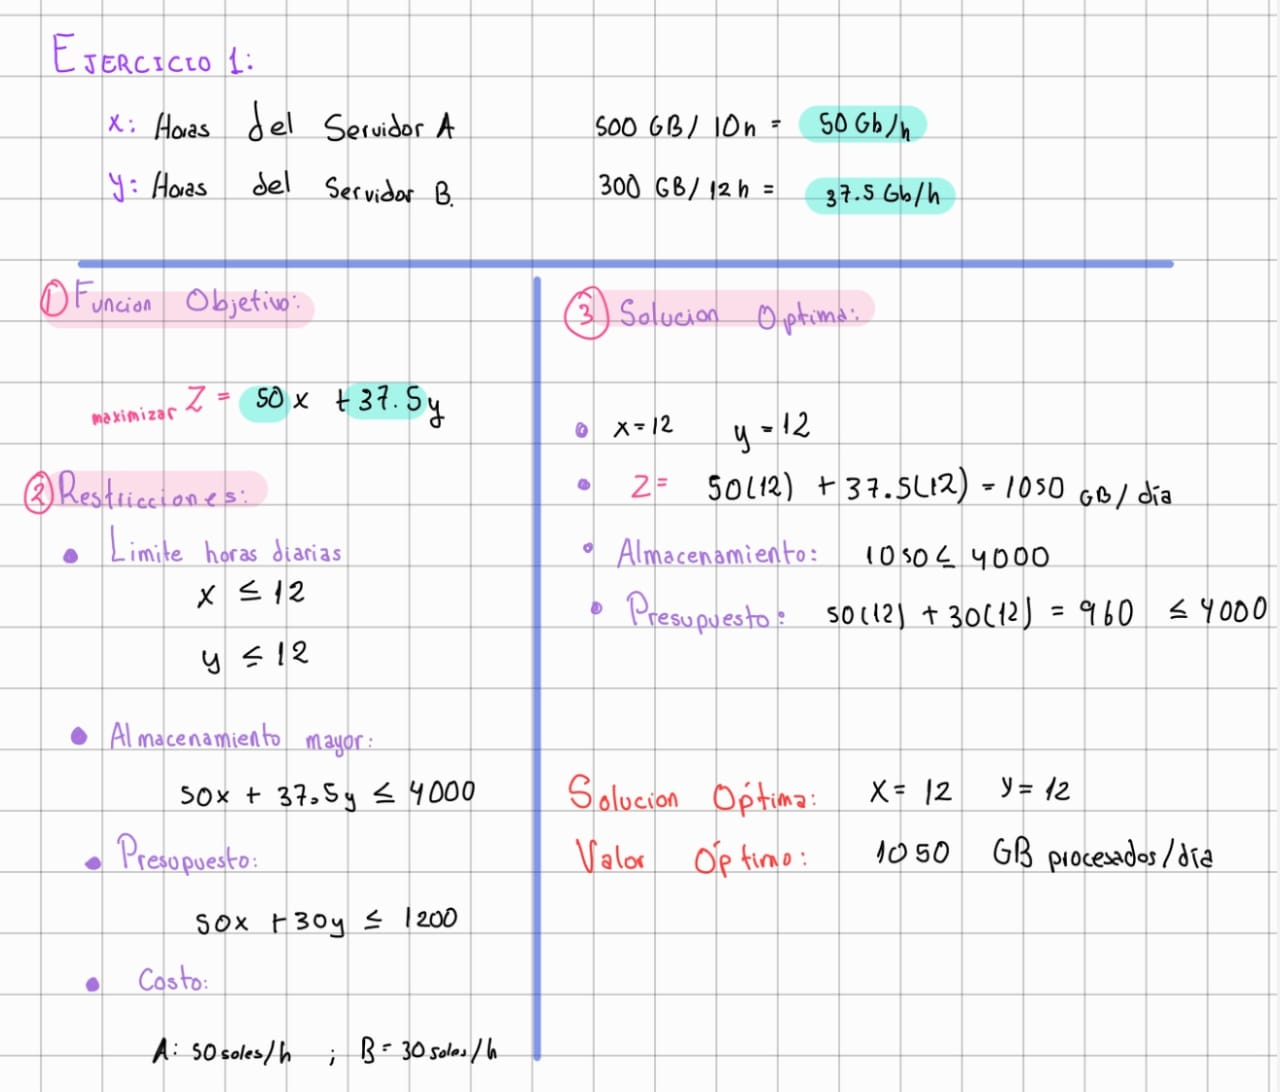
\includegraphics[width=1\textwidth]{ejercicio1.jpg}
    
    \label{fig:etiqueta}
\end{figure}



\vspace{0.5cm}


\textbf{Pregunta 2:}

Una empresa de seguridad monitorea sistemas de videovigilancia y debe analizar imágenes de alta resolución. Tiene dos centros de procesamiento: Centro A y Centro B. El Centro A puede analizar 80 imágenes por hora, y el Centro B puede analizar 100 imágenes por hora. Debido a los costos de mantenimiento, el Centro A no puede operar más de 10 horas al día y el Centro B no puede operar más de 12 horas al día. El sistema debe procesar al menos 1200 imágenes al día, y cada centro tiene un límite de almacenamiento de 600 imágenes al día. El objetivo es minimizar el número de horas de operación de ambos centros, asegurando que el número mínimo de imágenes procesadas sea alcanzado.

\begin{figure}[h]
    \centering
    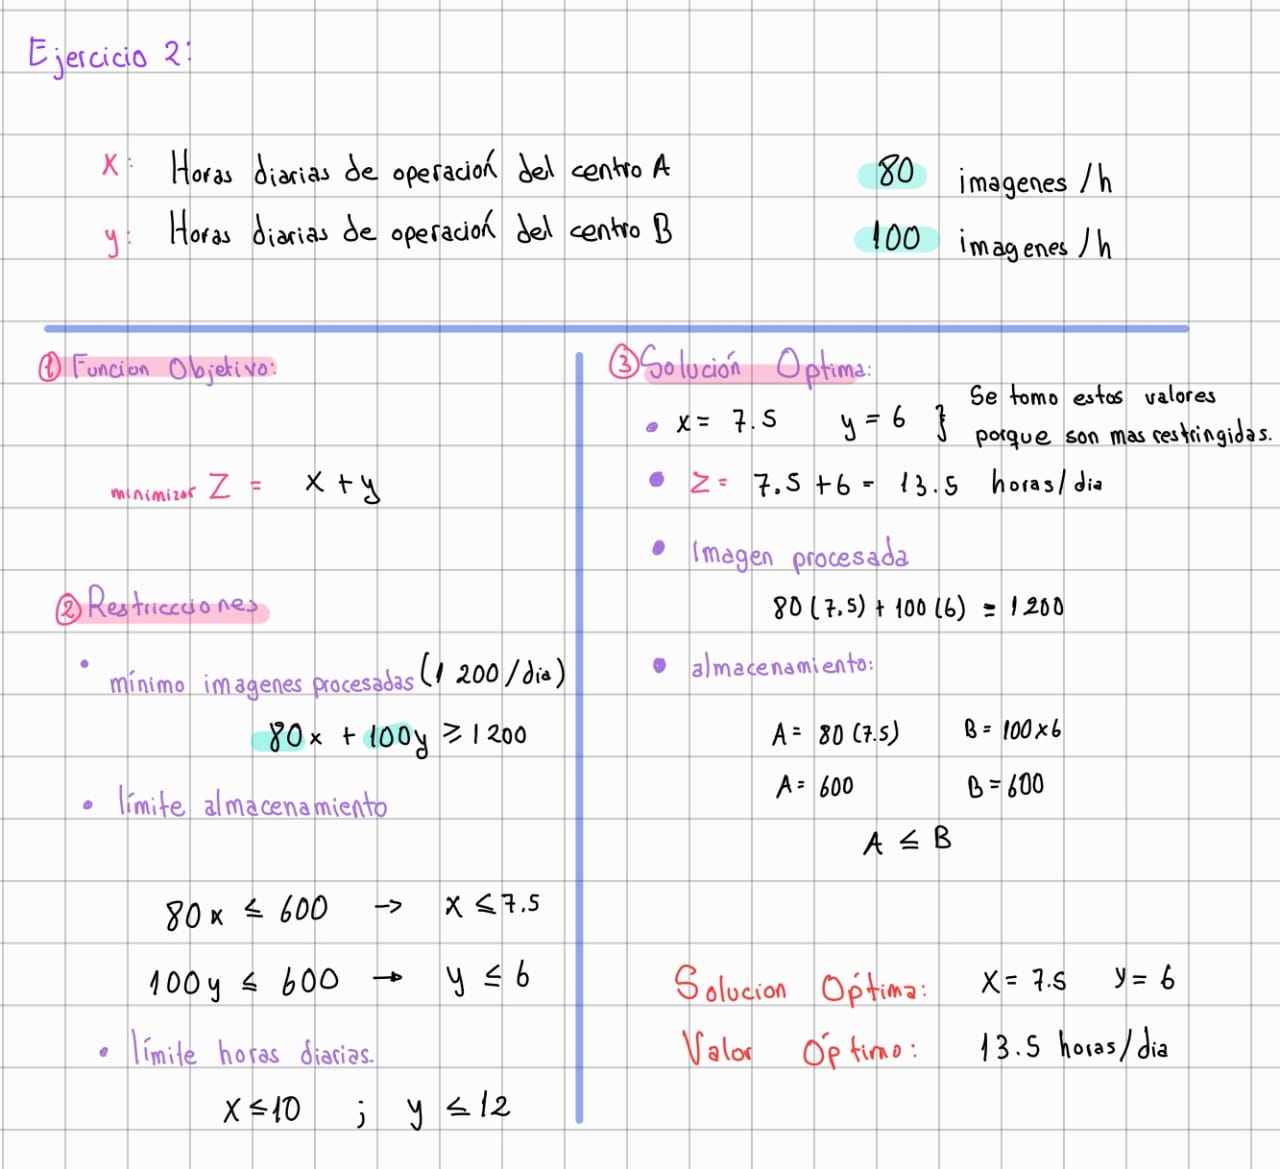
\includegraphics[width=1\textwidth]{ejercicio2.jpg}
    
    \label{fig:etiqueta}
\end{figure}

\end{document}
